\chapter{Resultado das Avaliações}
  
  Essa seção apresenta o resultados das avaliações feitas ao longo do projeto.
  
  \section{Avaliações do protótipo de papel}
     
     Para se realizar a avaliação do protótipo de papel, foi solicitado a 5 usuários com um perfil comum
     e compatível com a proposta do aplicativo (frequentadores de eventos), que realizassem dois cenários para a avaliação:
  
    \begin{itemize}
	\item A - Criar uma notificação com data e hora definidos.
	\item B - Gerenciar (edição e exclusão) suas notificações agendadas.
    \end{itemize}
     
    \noindent
    \textbf{Itens do questionário aplicado}
        
        Abaixo se encontram as perguntas, provenientes do questionário ASQ, que foram utilizadas após a realização
        de cada uma das atividades solicitadas no protótipo de papel:
        
	\begin{enumerate}
	\item No geral, estou satisfeito com a facilidade de completar das atividades neste cenário.
	
	\item No geral, estou satisfeito com a quantidade de tempo que levei para completar as atividades neste cenário.
	
	\item No geral, estou satisfeito com a informação de suporte (ajuda on-line, mensagens, documentação) fornecida
	  enquanto completava as atividades.
	\end{enumerate}
     
	É importante salientar que as questões tinham como opção de resposta de 1 a 7 e a opção “Não se aplica”,
	sendo que 1 significa que o usuário concorda fortemente com o que está sendo perguntado e 7 que o usuário
	discorda fortemente.
  
    \subsection{1ª iteração de avaliação}
        
          A tabela \ref{opnioes1iteracao} descreve o \textit{feedback} dos usuários com os pontos que faltaram na aplicação:
	
  \begin{table}[h]
  \centering
  \begin{tabular}{|m{1.5cm}||m{15cm}|}
    \hline
    \textbf{Usuário} & \textbf{Sentiu falta de:}\\
    
    \hline                               
    1 & 
      \begin{itemize}
	\item Um campo para escolher a cidade do evento na tela de escolher para quando deseja a notificação.
	\item Mensagem de confirmação de exclusão de uma notificação.
      \end{itemize}\\

    \hline                               
    2 & 
      \begin{itemize}
	\item Mensagem de notificação da perda dos dados caso queira voltar para uma tela anterior.
	\item A possibilidade de escolher um intervalo de horário para a notificações, ao invés de um horário fixo.
	\item Ao invés de colocar a mensagem de confirmação do salvamento de uma notificação em uma tela separada, colocar como uma mensagem sobrepondo a mesma tela.
	\item As notificações agendadas poderiam aparecer logo na página inicial.
      \end{itemize}\\
    
    \hline                               
    3 & 
      \begin{itemize}
	\item Uma melhor visualização do campo que exibe as notificações adicionadas.
	\item Lista de notificações agendadas mais centralizada.
	\item Símbolo de “Retirar tema” mais intuitivo.
	\item Caixinha de “Mais temas” na tela de edição.
      \end{itemize}\\
    
    \hline                               
    4 & 
    \begin{itemize}
      \item Especificação que a notificação de horário é referente a notificação.
      \item Melhorar símbolo de “menos” na tela de “Editar notificação”.
    \end{itemize}\\
    
    \hline                               
    5 & 
    \begin{itemize}
      \item Espaço para comentários sobre uma notificação. Ex: Comprar ingresso para a tia Tânia.
    \end{itemize}\\
    
    \hline
  \end{tabular}
  \caption{Opniões dos usuários na 1ª iteração de avaliação.}
  \label{opnioes1iteracao}
  \end{table}
  
  Na figura \ref{resposta_asq_1iteracao} se encontram as respostas ao questionário ASQ pelos cinco usuários avaliados.

  \begin{figure}[!htb]
  \centering
  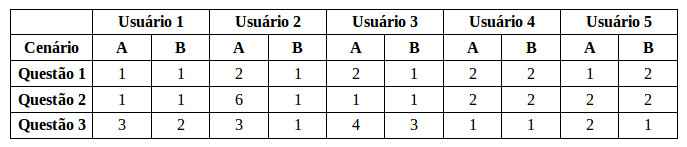
\includegraphics[scale=0.6]{figuras/nota1avaliacao.jpg}
  \caption{Resposta dos usuários ao questionário ASQ na primeira avaliação do protótipo de papel}
  \label{resposta_asq_1iteracao}
  \end{figure}
    
    \pagebreak
    \subsection{2ª iteração de avaliação}
    
  \pagebreak
  \subsection{Análise dos resultados obtidos na avaliação}
     
    De modo geral, o feedback recebido foi positivo e por ter sido adotado o questionário ASQ foi obtido um retorno
    capaz de fornecer uma medição mais precisa a medida que o projeto for evoluindo. Também por meio do uso do 
    questionamento sobre o que foi sentido falta, foi obtido um feedback rápido sobre a opinião do usuário em
    relação as melhorias necessárias.
